\documentclass[../main.tex]{subfiles}
\begin{document}

\section{Ground Truth for Performance Evaluation}
\label{sec:ground_truth}
To evaluate the performance of the Large Language Model (LLM) based system in automating administrative regularity checks, a ground truth dataset was established. This dataset serves as the benchmark representing the correct evaluation outcomes as determined by human expertise.

The ground truth was constructed based on a selected set of administrative acts: three acts (\textit{determine}) from the Municipality of Lucca and one act from the Municipality of Olbia. These acts were evaluated against their corresponding checklists, resulting in approximately 60 manually verified checklist points.

Establishing this ground truth was made possible through the collaboration with Promo PA Fondazione, which facilitated contact with a professional experienced in municipal administrative regularity control. This expert manually reviewed each selected administrative act and meticulously completed the associated checklists according to standard procedures. These human-generated evaluations constitute the "gold standard" against which the LLM's automated assessments were compared. The comparison allowed for quantitative measurement of the automated system's performance in replicating human judgment for this specific administrative task.

It is widely acknowledged within AI evaluation that static benchmarks inadequately capture the complexities and risks of LLMs in real-world applications; consequently, human interaction evaluations (HIEs), which assess the process and outcomes of human-model engagement, are essential for understanding true performance and bridging the sociotechnical gap in specific use contexts like administrative control. This approach is critical as performance in isolated tests often fails to predict outcomes when models interact with or replace human processes \cite{ibrahimStaticAIEvaluations2024}.


\section{Output Processing: Checklist Selection Agent}
\label{sec:output_choose_agent}
The primary function of the first LLM agent was to select the single most appropriate checklist for a given administrative act (\textit{determina}) from a predefined list. The prompt designed for this agent (detailed in Appendix \ref{appendix:prompts_choose}) explicitly instructed the LLM to output \textbf{only} the name (\texttt{NomeChecklist}) of the selected checklist (e.g., "Determine", "Contratti", "Affidamento Diretto"). Optional brief notes were permitted but the core expected output was strictly the checklist name.

However, LLMs can sometimes produce outputs that deviate from strict formatting instructions, potentially including introductory phrases, explanations for the choice, or concluding remarks. To ensure the system could reliably use the agent's selection, a straightforward text processing step was implemented. This step focused on extracting the intended checklist name from the raw text generated by the LLM, discarding any extraneous content. This ensured that only the valid \texttt{NomeChecklist} identifier was passed on for the subsequent checklist answering phase or for evaluation purposes, maintaining the workflow's integrity even with minor variations in the LLM's verbosity.

\section{Output Processing: Checklist Answering Agent}
\label{sec:output_answer_agent}
The second LLM agent was tasked with evaluating the administrative act against each point of the selected checklist. The prompt (detailed in Appendix \ref{appendix:prompts_answer}) required the LLM to provide a categorical assessment for each checklist point using one of three predefined labels: "SI" (compliant), "NO" (non-compliant), or "NON PERTINENTE" (not relevant)[. The prompt explicitly requested this evaluation in a specific format: \texttt{RISPOSTA GENERALE : [SI, NO, NON PERTINENTE], [spiegazione sintetica se necessaria]}.

Despite these instructions, practical experimentation revealed that the raw output from the LLMs often contained additional text beyond the core categorical answer and the optional brief explanation. This could include conversational filler, restatements of the checklist point, detailed justifications even when not required, or slight variations in the output structure (e.g., using different casing or omitting the "RISPOSTA GENERALE :" prefix).

To enable automated comparison against the human-generated ground truth and ensure consistent data for analysis, it was crucial to standardize these potentially verbose or inconsistently formatted responses. Therefore, a response parsing mechanism was implemented using regular expressions (\textit{regex}). This mechanism, encapsulated in the "analize\_response" function within the "ChecklistCompiler.py" program, was designed to robustly identify and extract only the core categorical answer ("SI", "NO", or "NON PERTINENTE") from the LLM's raw text output, ignoring surrounding text and handling minor formatting variations. The resulting standardized, single-word answer (stored as the 'Simple' value in evaluation dataframes) provided the clean, consistent data necessary for the performance metric calculations presented in Section \ref{sec:performance_metrics_eval}.


\section{Performance Metrics}
\label{sec:performance_metrics_eval}

To quantitatively assess the LLM-based system's performance against the established ground truth, several standard evaluation metrics for classification tasks were employed. The primary goal was to measure how accurately the system could replicate the human expert's evaluation for each checklist point, classifying it as compliant ('SI'), non-compliant ('NO'), or not relevant ('NON PERTINENTE').



\begin{itemize}
    
    \item \textbf{Accuracy}: This metric measures the overall correctness of the LLM's predictions. It is calculated as the ratio of correctly classified checklist points (where the LLM's answer matches the ground truth) to the total number of checklist points evaluated.
    
    \item \textbf{Balanced Accuracy}: To address potential class imbalance, balanced accuracy was also computed. It calculates the average accuracy obtained on each class individually. It is the average of recall obtained on each class, providing a better measure of performance when the number of 'SI', 'NO', and 'NON PERTINENTE' cases in the ground truth is uneven.

    \item \textbf{Confusion Matrix}: A confusion matrix provides a detailed breakdown of prediction results. It is a table showing the counts of true positive (TP), true negative (TN), false positive (FP), and false negative (FN) predictions for each class ('SI', 'NO', 'NON PERTINENTE'). This allows for a granular analysis of where the model succeeds and fails (e.g., does it confuse 'NO' with 'SI' often?).

    \item \textbf{F1-Score}: The F1-score is the harmonic mean of precision and recall, providing a single metric that balances both concerns. A high F1-score indicates that the model has both low false positives and low false negatives. The weighted F1-score averages the F1-score for each class, weighted by support.
    

\end{itemize}

These metrics collectively offer a comprehensive view of the LLM's performance, highlighting not only its overall accuracy but also its reliability in identifying specific compliance outcomes and handling potential imbalances in the data.


\subsection{Accuracy}
The graphs illustrate the accuracy  of different LLM families (Llama, Mistral, GPT) across temperature settings ranging from 0.0 to 1.0. A clear trend emerges where the GPT models (green bars) consistently outperform the Llama (blue bars) and Mistral (orange bars) families in terms of raw accuracy at most temperature settings. Accuracy for some models, particularly GPT-4o, tends to be highest at lower temperatures (e.g., 0.0, 0.2) and decreases slightly or becomes more variable at higher temperatures. Mistral and Llama models show varying performance, with Mistral generally achieving higher accuracy than Llama models across several temperatures.

When comparing the best-performing model from each family, GPT-4o maintains the highest accuracy, especially at lower temperatures. "Mistral v0.3 7B" shows competitive accuracy, particularly at mid-range temperatures (e.g., 0.6), while the best Llama models lag behind the other two families. The impact of temperature appears less predictable for Mistral and Llama compared to GPT-4o, where lower temperatures yield peak accuracy.

\begin{figure}[H]
    \caption{Models accuracy bar graph, grouped by family of models}
    \label{fig:Accuracy}
    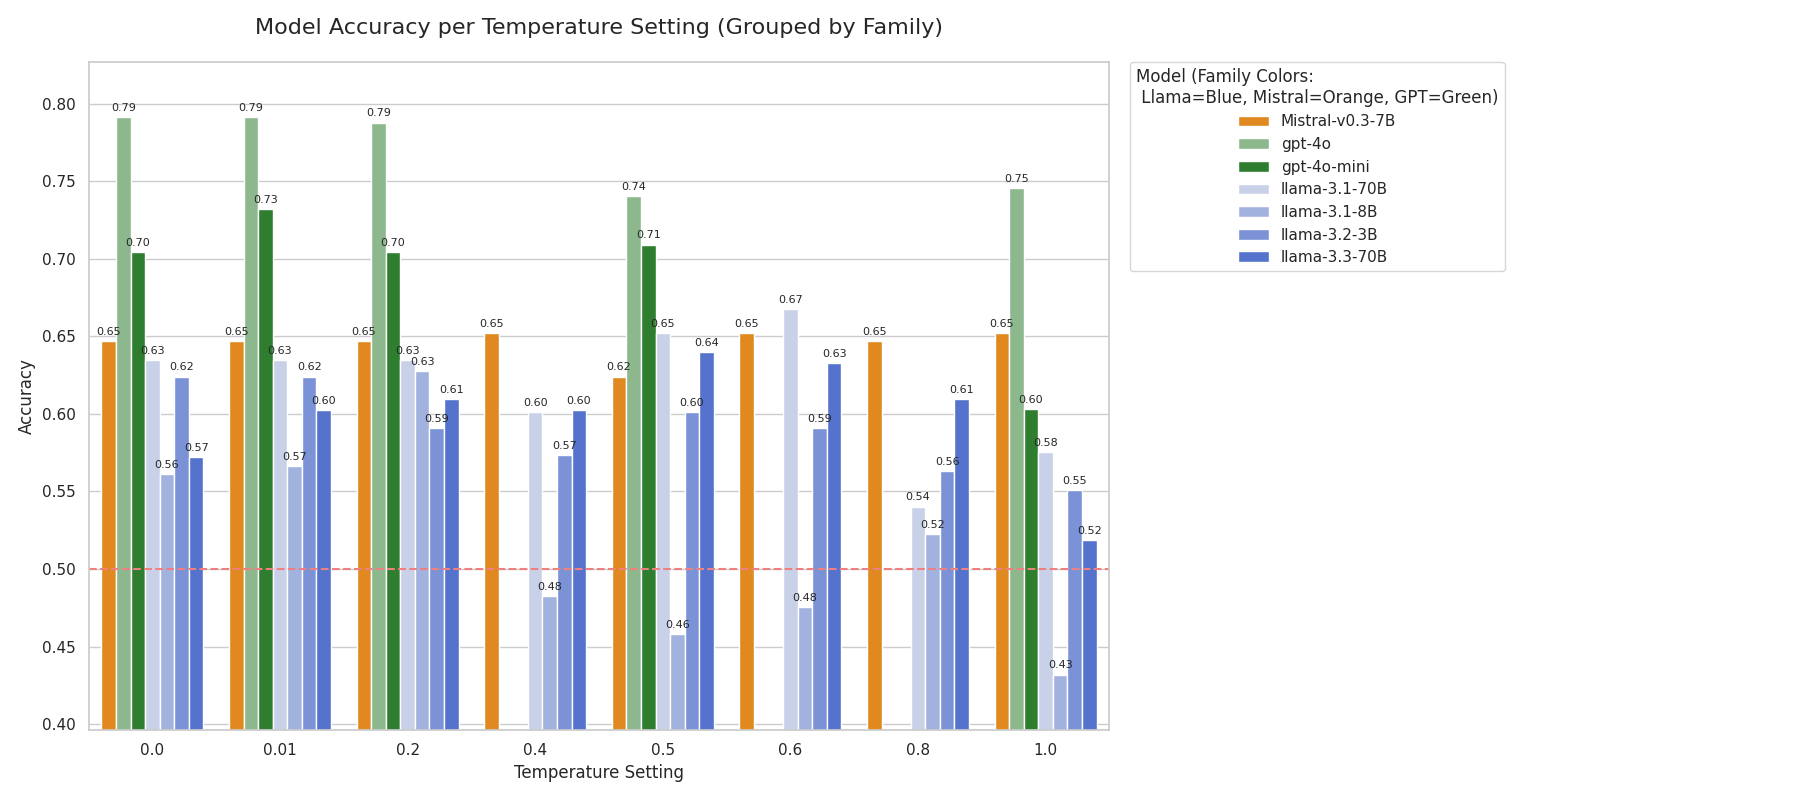
\includegraphics[width=\textwidth]{Graphs/Model Accuracy final.png}
\end{figure}

\begin{figure}[H]
    \caption{Models accuracy bar graph, using the best for each family of models}
    \label{fig:Accuracy_Best}
    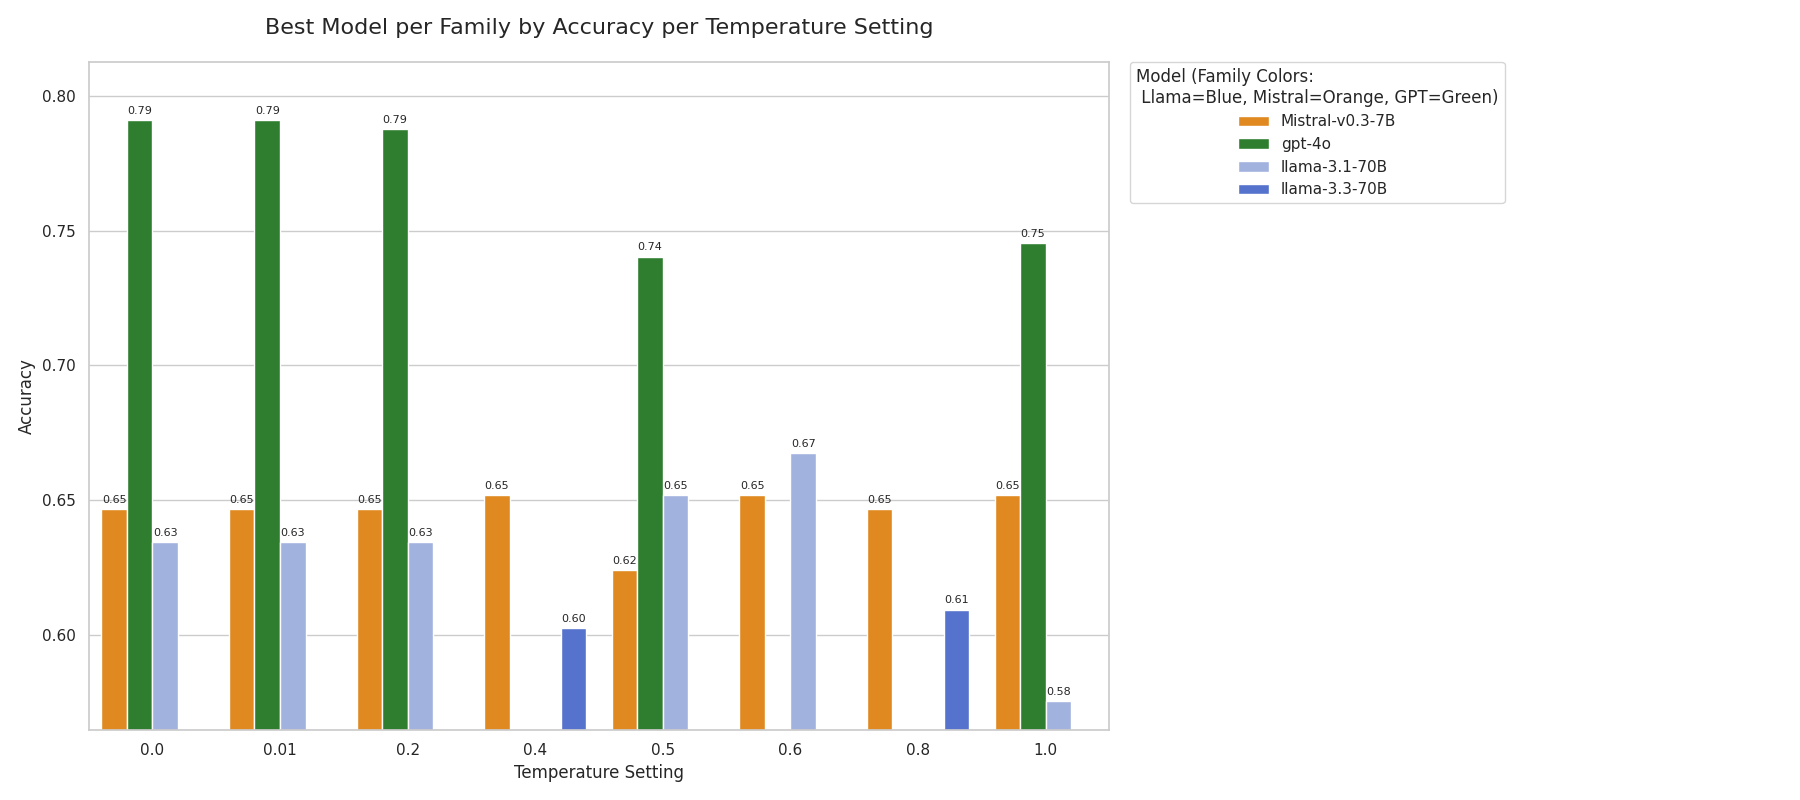
\includegraphics[width=\textwidth]{Graphs/Best_Accuracy.png}
\end{figure}


\subsection{Balanced Accuracy}
The graph presenting Balanced Accuracy reveals performance trends across model families and temperature settings. Balanced accuracy is calculated as the average of recall obtained on each class ("SI", "NO", "NON PERTINENTE") individually. This metric is particularly important because the ground truth dataset appears to be imbalanced, likely containing a significantly higher number of "SI" (compliant) instances compared to "NO" (non-compliant) and "NON PERTINENTE" (not relevant) instances, as suggested by the confusion matrices and the nature of compliance checks.

In such imbalanced scenarios, standard accuracy can be misleadingly high if a model simply performs well on the dominant "SI" class while failing to correctly identify the rarer, but potentially more critical, "NO" or "NON PERTINENTE" cases. Balanced accuracy mitigates this by giving equal importance to the performance on each class. Consequently, if models struggle more with the minority classes (like "NO"), the balanced accuracy scores may appear lower than the standard accuracy scores. This difference highlights that while overall correctness (standard accuracy) might seem high, the model's ability to reliably detect non-compliance or irrelevance might be weaker.

Observing the graph, the GPT family generally maintains the highest balanced accuracy, suggesting a more consistent performance across all outcome types compared to Mistral and Llama families. While the absolute scores might be slightly lower than standard accuracy for some models, balanced accuracy provides a crucial and more realistic evaluation of the models' effectiveness in handling the uneven distribution of compliance outcomes inherent in this administrative task. It underscores the importance of evaluating models not just on overall correctness but on their capability across all classification categories.

\begin{figure}[H]
    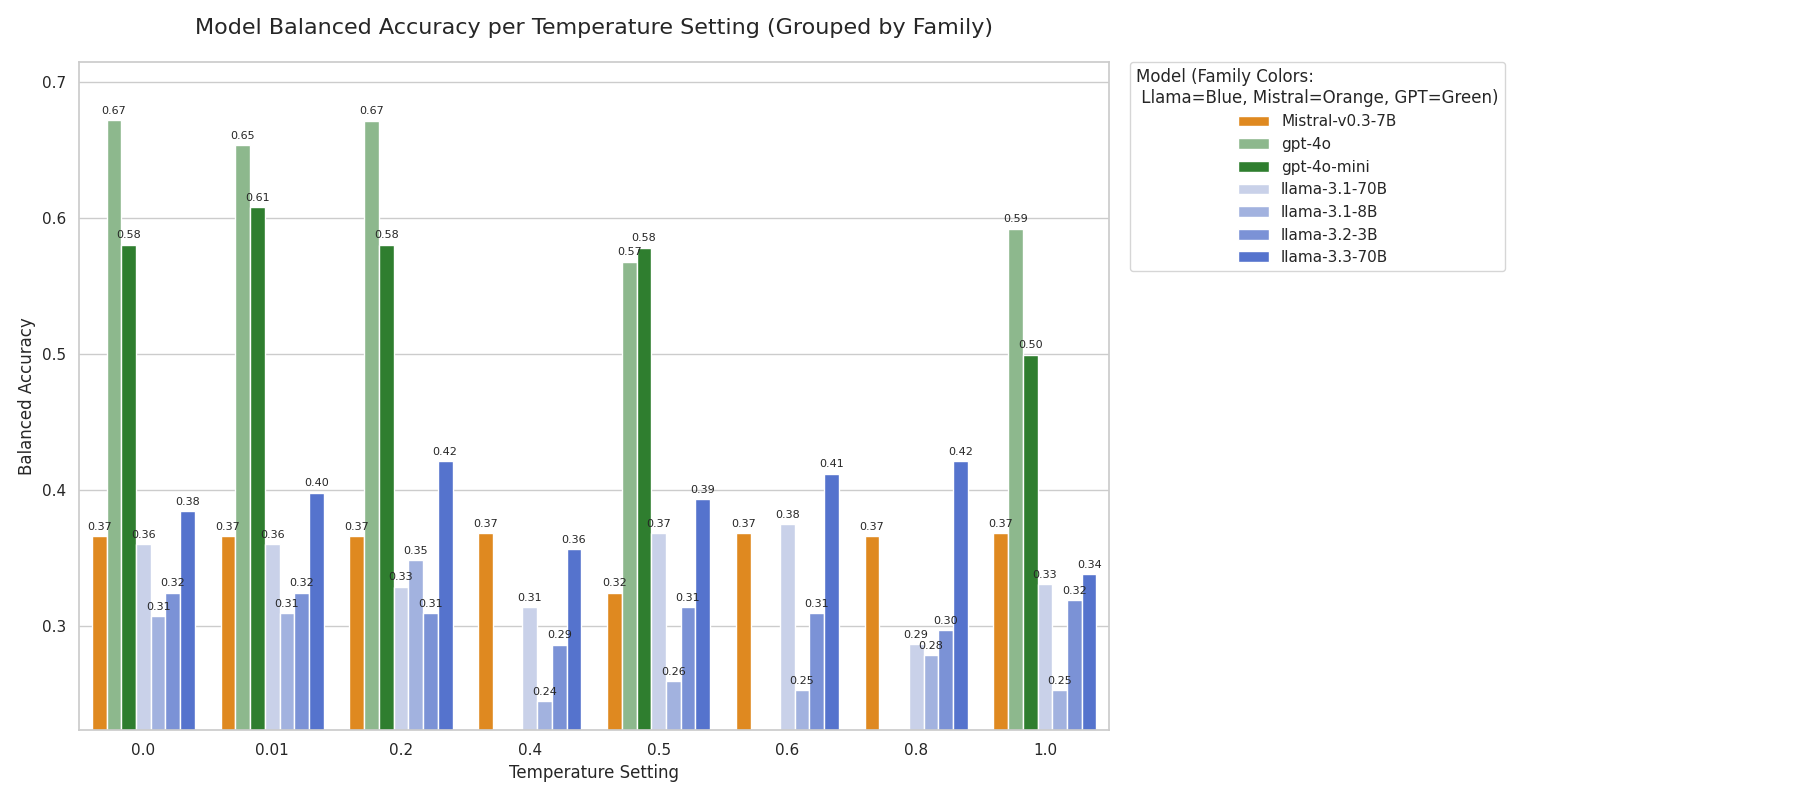
\includegraphics[width=\textwidth]{Graphs/Balanced Accuracy.png}
\end{figure}

\subsection{F1 Score}
The F1-Score graph, which balances precision and recall, further reinforces the performance hierarchy. GPT models generally exhibit the highest F1 scores, suggesting they are effective at minimizing both false positives and false negatives. The trends across temperature settings are consistent with the accuracy and balanced accuracy results, highlighting the strong performance of GPT-4o, particularly at lower temperatures. Mistral models show respectable F1 scores, while Llama models generally score lower.

\begin{figure}[H]
    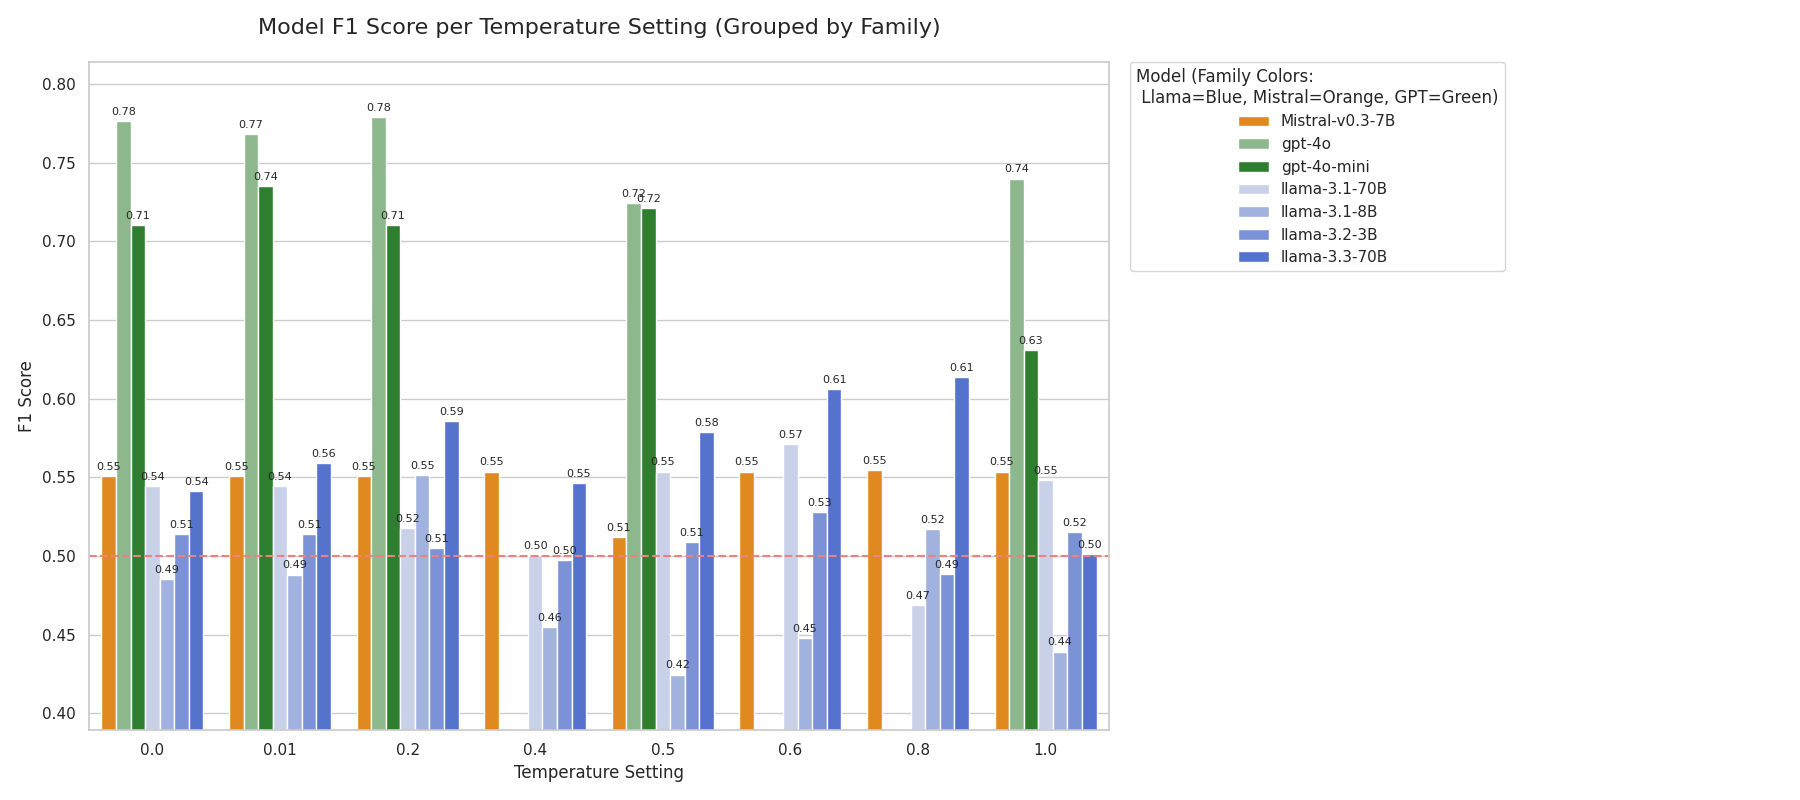
\includegraphics[width=\textwidth]{Graphs/Model f1 Scores.png}
\end{figure}

\newpage
\subsection{Confusion Matrix}

\subsubsection{GPT 4o Confusion Matrix}
\begin{wrapfigure}{L}{0.70\textwidth}
    \centering
    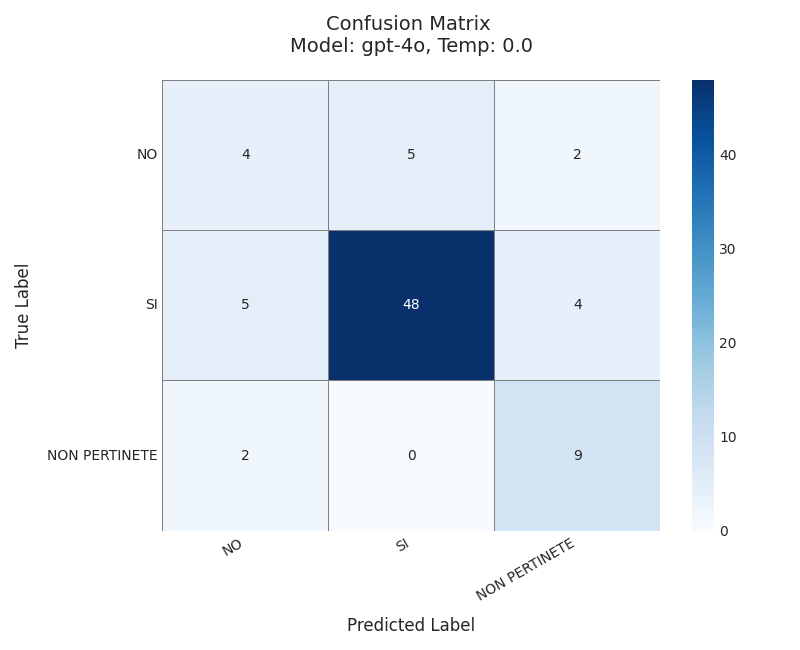
\includegraphics[width=0.70\textwidth]{Graphs/Confusion Matrix GPT 4o.png}
\end{wrapfigure}


\textbf{GPT-4o (temperature 0.0)}: This model shows high accuracy, correctly classifying a large number of "SI" cases (48 true positives). However, it exhibits some confusion, notably misclassifying 5 "NO" cases as "SI" (false positives for "SI") and 4 "SI" cases as "NON PERTINENTE" (false negatives for "SI"). It also misclassified 2 "NON PERTINENTE" cases as "NO".


\begin{wrapfigure}{r}{0.70\textwidth}
    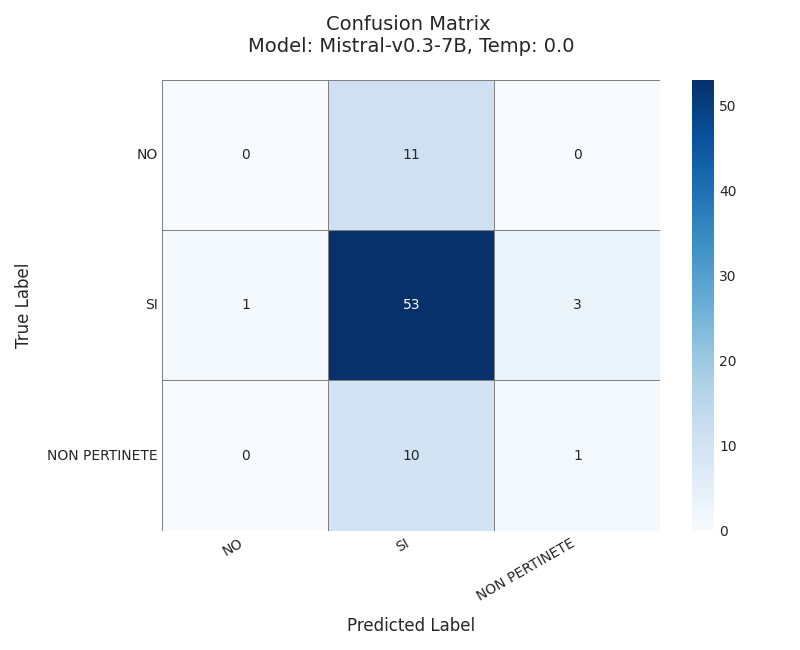
\includegraphics[width=0.70\textwidth]{Graphs/Confusion Matrix Mistral.png}
\end{wrapfigure}

\textbf{Mistral-v0.3-7B (temperature 0.0)}: This model also performs reasonably well, correctly identifying 34 "SI" cases. Its primary errors include misclassifying 11 "NO" cases as "SI" and 10 "NON PERTINENTE" cases as "SI" (significant false positives for "SI"). It also misclassified 7 "SI" cases as "NON PERTINENTE".

\textbf{Summury}: Both models perform best at identifying the "SI" (compliant) category. However, they struggle more with distinguishing between "NO" (non-compliant) and "NON PERTINENTE" (not relevant), and both tend to incorrectly classify actual "NO" or "NON PERTINENTE" cases as "SI" more often than other error types. This suggests potential challenges in correctly identifying non-compliance or irrelevance compared to confirming compliance. 


% Include bibliography only when compiling this subfile independently
\ifSubfilesClassLoaded{
    \bibliographystyle{sapthesis}
    \bibliography{Tesi}
}{}

\end{document}